\section{差分方程模型}
\subsection{微分方程应用背景}
\begin{enumerate}
\item 研究问题是离散的
\item 连续数学模型离散化
\end{enumerate}
\subsection{差分方程}
\subsubsection{数列的差分}
{\heiti 定义:}\par
数列$\{a_n\}$相当于定义在正整数集上的函数:$\mathbb{Z}^+ \rightarrow \mathbb{R}$
{\renewcommand\labelenumi{例\theenumi}
\begin{enumerate}
\item $a_n = \frac{n}{n+1}, n = 1, 2, \cdots$
\item Fibonacci数列(黄金分割数列、兔子数列)
\[
\text{数列定义:}a_1 = 1, a_2 = 1, a_n = a_{n-1}+a_{n-2}, n>2
\]\[
\lim_{n\to\infty} \frac{a_n}{a_{n+1}} = \frac{\sqrt{5}-1}{2} \approx 0.618\text{ (黄金分割比)}
\]
繁殖模型:一对幼兔出生一月后成年,再过一月产下一对幼兔。

起始:一对幼兔

\begin{tabular}{ccccc}
\hline
月数 & 0 & 1 & 2 & 3 \\
\hline
幼兔 & 1 & 0 & 1 & 1 \\
\hline
成兔 & 0 & 1 & 1 & 2 \\
\hline
总数 & 1 & 1 & 2 & 3 \\
\hline
\end{tabular}
\end{enumerate}}\par
{\heiti 数列的差分}\par
\[\Delta a_n := a_{n+1} + a_n, n = 1, 2, \cdots\]\par
{\heiti 差分的意义}
\begin{enumerate}
\item 平均速率\\
$S(n)$:$n$时刻的旅程

$S(n)-S(n-1) = \frac{S(n)-S(n-1)}{1}$:$n$时刻平均速率
\item 斜率\\
$f(n)$:整数节点处的函数取值
$f(n)-f(n-1) = \frac{f(n)-f(n-1)}{1}$:$n-1$、$n$两点间连线的斜率,如下图所示:\\
\begin{center}
\begin{tikzpicture}
%坐标系
\draw[->] (-0.5,0) -- (2.5,0);
\draw[->] (0,-0.5) -- (0,2.5);
%定位线
\draw[dashed] (0.5,0) -- (0.5,0.5);
\draw[dashed] (2,0) -- (2,0.5);
%图形
\draw (0.5,0.5) -- (2,0.5);
\draw (2,0.5) -- (2,1.5);
\draw (0.5,0.5) -- (2,1.5);
\node[above] (n-1) at (0.5,0.5) {$\scriptscriptstyle f(n-1)$};
\node[right] (n) at (2,1.5) {$\scriptscriptstyle f(n)$};
\end{tikzpicture}
\end{center}
\end{enumerate}
\subsubsection{差分方程}
{\heiti 定义}\par
数列中任意一项与前几项的关系式。\par
例:$a_n = a_{n-1}+a_{n-2}$\par
{\heiti 差分方程的阶}\par
方程中最大下标与最小下标之差。\par
{\heiti 差分方程类别}\par
\begin{itemize}
\item 常系数差分方程:
\[
a_n + c_1 a_{n-1} + c_2 a_{n-2} + \cdots  + c_k a_{n-k} = f(n) (n>k)\\
c_i\text{为常值}\]
\item 变系数差分方程:差分方程中$c_i$为函数
\end{itemize}
\subsubsection{差分方程的求解}
{\renewcommand\theenumi{\Roman{enumi}}
\begin{enumerate}
\item 理论分析:\\
分析差分方程解的存在性、稳定性等性质。可参考线性代数I-A中的内容和其他相关参考资料
\item 数值求解:\\
迭代求解,关键在于选取合适的初值条件。
\end{enumerate}
\subsection{连续模型的离散化}
\subsubsection{微分的离散化}
例:已知$f\in \mathbf{C}^1[a,b]$,且仅知道$f(x_k), k=0, 1, 2, \cdots  ,n+1, a\leq x_0<\cdots<x_k\leq b$,求$f'(x_k)$。

方法:数值微分
\begin{enumerate}
\item 向前差分:$f'(x_k) = \frac{f(x_{k+1})-f(x_k)}{x_{k+1}-x_k}$
\item 向后差分:$f'(x_k) = \frac{f(x_k)-f(x_{k-1})}{x_k-x_{k-1}}$
\item 中心差分:向前、向后差分求算术平均。近似效果更好。
\end{enumerate}
\subsubsection{积分的离散}
计算$I = \int_a^b f(x)\,\mathrm{d}x$ ——数值积分公式
\begin{enumerate}
\item 复化梯形公式:用梯形面积近似曲边梯形面积,在区间上进行线性插值拟合。
\begin{center}
\begin{tikzpicture}
%坐标系
\draw[->] (-0.5,0) -- (5.5,0);
\draw[->] (0,-0.5) -- (0,4);
\node[below left] (O) at (0,0) {$O$};
\node[right] at (5.5,0) {$x$};
\node[above] at (0,4) {$y$};
%函数曲线
\draw[domain = 0.1:5.2] plot (\x, {2*ln(\x+1)});
%坐标轴标记
\foreach \t in {0.5, 1.5, 2.5, 3.5, 4.5} {
	\draw (\t,-0.05) -- (\t,0.05);
}
\node[above] at (0.5,0) {$a$};
\node[above] at (4.5,0) {$b$};
\node[below] at (0.5,0) {$x_0$};
\node[below] at (1.5,0) {$x_1$};
\node[below] at (2.5,0) {$x_k$};
\node[below] at (3.5,0) {$x_{k+1}$};
\node[below] at (4.5,0) {$x_n$};
%梯形
\draw (2.5,0) -- (2.5,{2*ln(3.5)});
\draw (3.5,0) -- (3.5,{2*ln(4.5)});
\draw (2.5,{2*ln(3.5)}) -- (3.5,{2*ln(4.5)});
\end{tikzpicture}
\end{center}
\[
I \approx \frac{h}{2}\sum_{k=0}^{n-1}\left[f(x_k)+f(x_{k+1})\right], h=b-a\]

\item 复化Simpson公式:利用$x_k, x_{k+1}, (x_k+x_{k+1})/2$三点对应的二次曲线拟合闭区间$[x_k,x_{k+1}]$上的函数图像。\[
x_{k+\frac{1}{2}} := \frac{x_k+x_{k+1}}{2}\]\[
I \approx \frac{h}{6}\sum_{k=0}^{n-1}\left[f(x_k)+4f(x_{k+\frac{1}{2}})+f(x_{k+1})\right]\]
\end{enumerate}
}MATLAB软件拥有微分、积分的数值计算和符号计算工具包。

\subsection{差分方程模型}
\subsubsection{市场经济中的“蛛网”模型}
{\heiti 模型图示}\par
\[
\xymatrix{
\fbox{供不应求}\ar[r]  & \fbox{价格上涨}\ar[r] & \fbox{产量增加}\ar[dd]\\
{} & \mbox{寻求平衡} & {}\\
\fbox{产量减少}\ar[uu] & \fbox{价格下降}\ar[l] & \fbox{供过于求}\ar[l]\\
}
\]\par
{\heiti 模型刻画}\par
$x_k$:$k$时刻商品数量

$y_k$:$k$时刻商品价格

需求关系:$y_k = f(x_k)\downarrow$

供应关系:$x_{k+1} = h(y_k)\uparrow\  \Longrightarrow y_k = g(x_k+1)$
\begin{center}
\begin{tikzpicture}
%坐标系
\draw[->] (-0.5,0) -- (3,0);
\draw[->] (0,-0.5) -- (0,3);
\node[right] at (3,0) {$x$};
\node[above] at (0,3) {$y$};
\node[below left] at (0,0) {$O$};
%图像
\draw[domain=2.9:0.4] plot (\x,{1/\x}) node[above]{$f$};
\draw[domain=0.1:2.6] plot (\x,{1/(3-\x)}) node[above]{$g$};
%稳定点
\coordinate[label = right:{  $\longrightarrow$稳定点}] (stable) at (1.5,{1/1.5});
\draw[dashed] (1.5,0) -- (1.5,{1/1.5});
\draw[dashed] (0,{1/1.5}) -- (1.5,{1/1.5});
\node[below] at (1.5,0) {$x_0$};
\node[left] at (0,{1/1.5}) {$y_0$};
\end{tikzpicture}
\end{center}
寻找稳定点:
\begin{figure}[H]
\centering
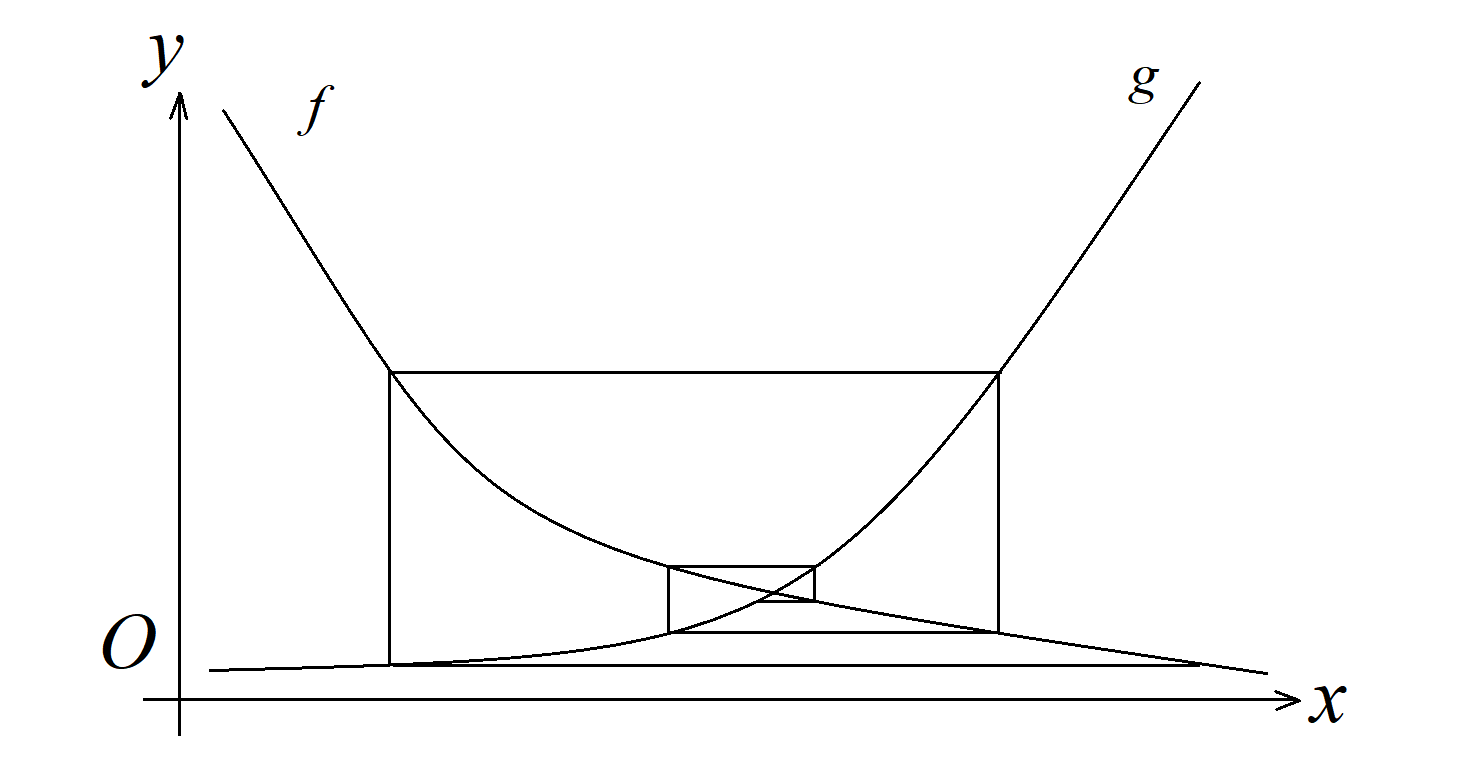
\includegraphics[width = 0.6\textwidth]{Figures/appro.png}
\caption{“蛛网”模型}
\end{figure}
分析:什么条件下可收敛至稳定点?
\begin{description}
\item[$\alpha$:] 商品数量减少一个单位对应价格上涨的幅度
\item[$\beta$:] 价格上涨一个单位对应供应量的增量
\end{description}
$\alpha>0,\text{  }\beta>0$
\begin{gather*}
y_k - y_0 = -\alpha(x_k - x_0)\\
x_{k+1} - x_0 = \beta(y_k - y_0)\\
\Longrightarrow x_{k+1}-x_0 = -\alpha\beta(x_k - x_0) = (-\alpha\beta)^k(x_1-x_0)\\
\text{稳定:}x_{k+1}-x_0 \longrightarrow 0 \Longrightarrow \alpha\beta<1
\end{gather*}
当$\alpha\beta\ge1$时,模型发散,此时需要政府宏观调控。

\section{储油罐的变位识别与罐容表标定}
\subsection{题目}
\begin{center}
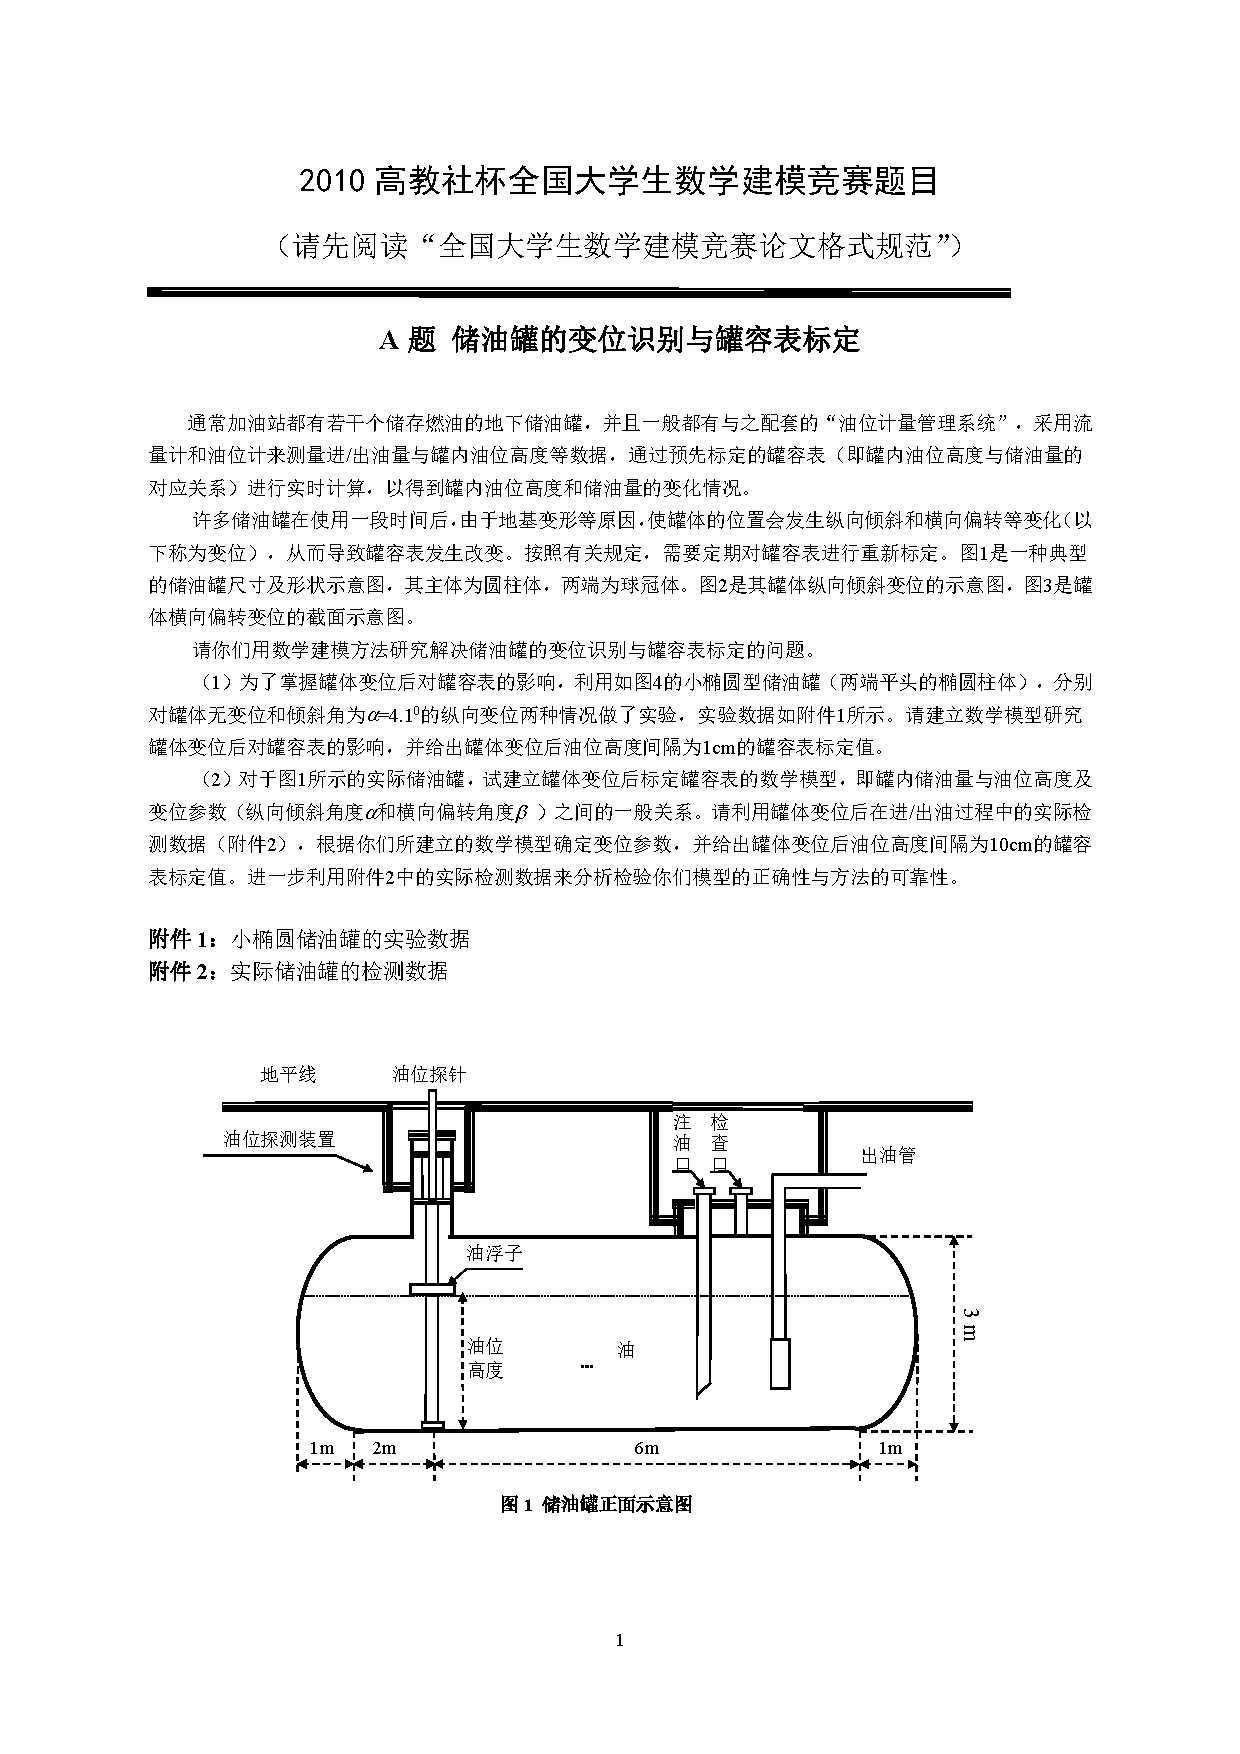
\includegraphics[page=1,scale=0.7]{Figures/2010A}
\includegraphics[page=2,scale=0.7]{Figures/2010A}
\end{center}
\subsection{模型假设}
\begin{enumerate}
\item 不考虑油罐由于温度压强等外力变化而引起的体积变化。
\item 油位探针被固定且油浮子的测量是准确的。
\end{enumerate}
\subsection{符号说明}
\begin{table}[htbp]
\begin{tabular}{@{}lll@{}}
\toprule
符号 & 说明 &  \\ \midrule
$L$ & 圆柱体长度 &  \\
$R$ & 圆柱体底面半径 &  \\
$h$ & 油位高度 &  \\
$R_0$ & 球冠体的半径 &  \\
$H_0$ & 球缺的高度 &  \\
$\beta$ & 横向偏转角 &  \\
$\alpha$ & 纵向偏转角 &  \\ \bottomrule
\end{tabular}
\end{table}
\subsection{建立数学模型}
\subsubsection*{储油罐的容积}
$$V\,=\,V_{\text{柱}}+2V_{\text{球缺}}\,=\,\pi R^2L+2\pi H^2(R_0-\frac{H}{3})$$
\subsubsection*{不发生形变时,$h$与容量的关系}
\begin{enumerate}
\item $h\leq R$时
    \begin{itemize}
    \item $V_\text{柱}(h)=\int_0^h2L\sqrt{R^2-(R-\tau)^2}{\mathrm{d}}\tau$
    \item $\theta=\arccos\left(\frac{R_0-H}{r_\text{圆}}\right)$
    \item $r_\text{圆}=\sqrt{R_0^2-(R-\tau)^2}$
    \item $V(h)=V_{\text{柱}}+2V_{\text{球缺}}$
    \end{itemize}

\item $h>R$时
    \begin{itemize}
    \item V(h)=V-V(2R-h)
    \end{itemize}
\end{enumerate}

\subsubsection*{只考虑横向偏转}
\begin{enumerate}
\item $h_\beta\neq R$时
    \begin{itemize}
    \item $h=R-(R-h_\beta)\cos\beta$
    \end{itemize}
\item $h_\beta\>R$时
    \begin{itemize}
    \item 思路与上同。
    \end{itemize}
\end{enumerate}
\subsubsection*{只考虑纵向偏转}
\begin{enumerate}
\item $h_\alpha=0$
\item $h_\alpha\in(0,(L-l)\tan\alpha)$
\item $h_\alpha\in((L-l)\tan\alpha,2R-l\tan\alpha)$
\item $h_\alpha\in(2R-l\tan\alpha,2R)$
\end{enumerate}
\subsubsection*{同时发生横向偏转与纵向偏转}
$h_\alpha=R-(R-h\beta)\cos\beta$
\subsection{模型的求解}
已知,$h(\alpha,\beta)$,可以算出体积$V(h,\alpha,\beta)$。
$$\Delta V_i\,=\,V(h_{i+1},\alpha,\beta)-V(h_i,\alpha,\beta)$$
于是
$$\min_{\alpha,\beta}\left\{\sum_i^{i'}(\Delta V_i-\Delta V_i')^2\right\}$$